\pagestyle{fancy}
\fancyhf{}
\renewcommand{\headrulewidth}{0pt}
\fancyfoot[C]{\leftmark}
\fancyhead[R]{\thepage}
\doublespacing
\chapter{Mechanical response of thermally processed inhomogeneous glass}\label{chap4}

\section{Introduction}

Response of amorphous solids to external shear has been extensively studied for last few decades \cite{nicolas2018deformation,ludovicRMP2017,larson}, to understand the process of mechanical failure from a fundamental perspective. Such insight will also help in improving the performance of existing applications and also in developing new applications. 

Under shear, glassy materials initially deform elastically with the linear increase in stress for small strain values but as the strain reaches some threshold, the measured stress shows an overshoot which is followed by a stress drop to reach a steady value eventually \cite{falkLanger98,gauravJRheo15,gauravPRE15}, for most ductile materials. Hence, a finite shear rate deformation will transform an amorphous solid glass to a homogeneously flowing fluid at sufficiently large strains. This transformation mechanism is still not properly understood at microscopic level. A key feature observed during the stress relaxation is the emergence of inhomogeneous flow patterns. Quite often, the inhomogeneities lead to formation of a band like structure with higher strain or mobility than the other parts \cite{golkia2020}. The material in the bands flow relatively more than the other part of the system, and these patters are called shear bands. In ductile materials, the formation of these bands start near the strain value where the stress overshoot happens and then these bands grow to cover the whole system when flow becomes completely homogeneous. In the context of metallic glasses, the understanding of shear banding becomes important to improve the ductility of the material. Also, in recent studies \cite{ozawa2018random,ozawa2020role}, it has been shown, the nature of shear band depends on the degree of annealing of the initial glassy sample. For better annealed glasses, a system spanning shear band is formed near the strain value where it shows a sharp stress drop.  

\section{Objective}
It has been already noted in many earlier studies, e.g. in the context of metallic glasses \cite{cheng2011intrinsic,tian2012approaching}, the shear band nucleation can be homogeneous or heterogeneous. The pure bulk materials without any manufacturing inhomogeneity, are expected to show homogeneous nucleation of shear bands i.e., whole material fail together. But, most of the materials in our day-to-day life have some manufacturing glitch, which cause nucleation of shear bands at specific locations. The prediction of the location where the shear band initiates, has not been completely possible. But many studies \cite{hieronymus2017shear,hassani2019probing} have proposed, shear bands are formed due to the accumulation of Eshelby quadrupoles formed by local stress or nonaffine displacement \cite{dasgupta2013yield,falkLanger98}. In general, it is found, soft regions tend to rearrange plastically and hence shear band nucleation happens from these soft regions. It has been shown in the work by Ozawa {\em et al.} \cite{ozawa2022rare}, how the microscopic failure starts from a synthetic soft region with the nucleation of shear band. Hence, one can ask a broader question in this context, can we design a material with predetermined failure pathway? We attempt to provide the answer to this question by proposing a thermal protocol based on the application of temperature gradient to generate glassy samples with spatial inhomogeneity of density and concentration such that the failure of these inhomogeneous samples always follows a specific pathway. In other words, our thermal protocol generate glassy samples with soft regions prone to mechanical failure and shear band nucleation.

It is very well known that applying thermal gradient to a liquid results a mass flux which leads to a spatial variation of concentration and density in the direction of gradient. As discussed in the previous chapter \cite{vaibhav2020response}, we have shown via simulations that how a glass-forming liquid responds to an externally applied temperature gradient. Since the structural relaxation process in supercooled state is slow but the timescales are finite enough such that after removing the externally applied thermal gradient, the liquid returns to the homogeneous state in a short time window. But due to very slow structural relaxation process in glassy state, the inhomogeneity created by the thermal gradient does not vanish completely even after removing the gradient. Hence, inhomogeneous glassy samples can be prepared by applying a thermal gradient pulse i.e., switching the gradient on for a small time window ({\em exposure time} $t_{\rm exp}$) and then switch this off \cite{vaibhav2020response}. In this work, we use a similar thermal protocol or thermal processing which prepares glassy samples with spatial inhomogeneity. Some part of these inhomogeneous samples are prone to mechanical failure and shear band nucleation.

\section{Model and methods}
The model that we have considered for the study in this chapter is the Kob-Andersen 80-20 (AB) binary Lennard-Jones mixture \cite{kob1995testing}. This is the same model that we have studied in previous chapter. The details related to this model can be seen in section-\ref{model} of Chapter-\ref{chap2}.

 The range of the interactions is set to $R_{c} = 2.5\sigma_{\rm{\alpha\beta}}$ with $\{\alpha,\beta\} \in \{A,B\}$. All measured quantities are expressed in LJ units, where lengths and energies are expressed in units of $\sigma_{\rm AA}$ and $\varepsilon_{\rm AA}$, respectively.  The unit of time is $\sqrt{{m\sigma_{\rm AA}^{2}}/\varepsilon_{\rm AA}}$. We have considered $N= 48 000$ particles in a three dimensional rectangular box with $L_x = L_y = 20$ and $L_z = 100$, and with periodic boundary conditions in all three directions to perform large-scale molecular dynamics simulation where equations of motion are integrated using velocity-Verlet algorithm in LAMMPS \cite{lammps} with time step $\Delta t = 0.005$. 
 
 At first, high temperature liquid is equilibrated at $T = 3.0$ which is then quenched to $T = 0.45$. Thr equilibrated independent configurations at $T = 0.45$ are finally quenched to lower temperatures $T_C$ below the $T_{\rm MCT} \approx 0.435$ and which subsequently aged for $t_{\rm age} = 10^4$.
 
 The method to apply the temperature gradient is same as we have followed in Chapter-\ref{chap3}. Just to remind, we mention the protocol briefly: extreme ends with width $L_z/20$ each (hot zone), maintained at temperature $T_H$ and central region with width $L_z/10$ (cold zone) is maintained at $T_C$. This local thermostatting is done using Langevin thermostat with a dissipation timescale of $\tau_d=0.5$ (check section-\ref{thermostat} in Chapter-\ref{chap2} for details on Langevin thermostat).
 
 As discussed above, after preparing the inhomogeneous glassy samples using the thermal protocol (to be discussed in the section below), they are sheared at constant shear rate $\dot{\gamma}$. To impose the shear by deforming the $xz$-plane in the $x$-direction, Lees-Edwards boundary conditions are utilised (more details to impose shear is discussed in Chapter-\ref{chap1}). DPD thermostat\cite{dpd} (check section-\ref{thermostat} in Chapter-\ref{chap2} for details on DPD thermostat) is applied during the shear to maintain the temperature at $T_C$.
 
 Before and after applying the temperature gradient, spatial profiles of various quantities like density, concentration, potential energy etc. are measured in 100 bins along $L_z$, to see the spatial variation of these quantities.

\section{Results}

\subsection{Preparing inhomogeneous glassy states}

%%%%%%%%%
\begin{figure*}[hbt!]
\centering
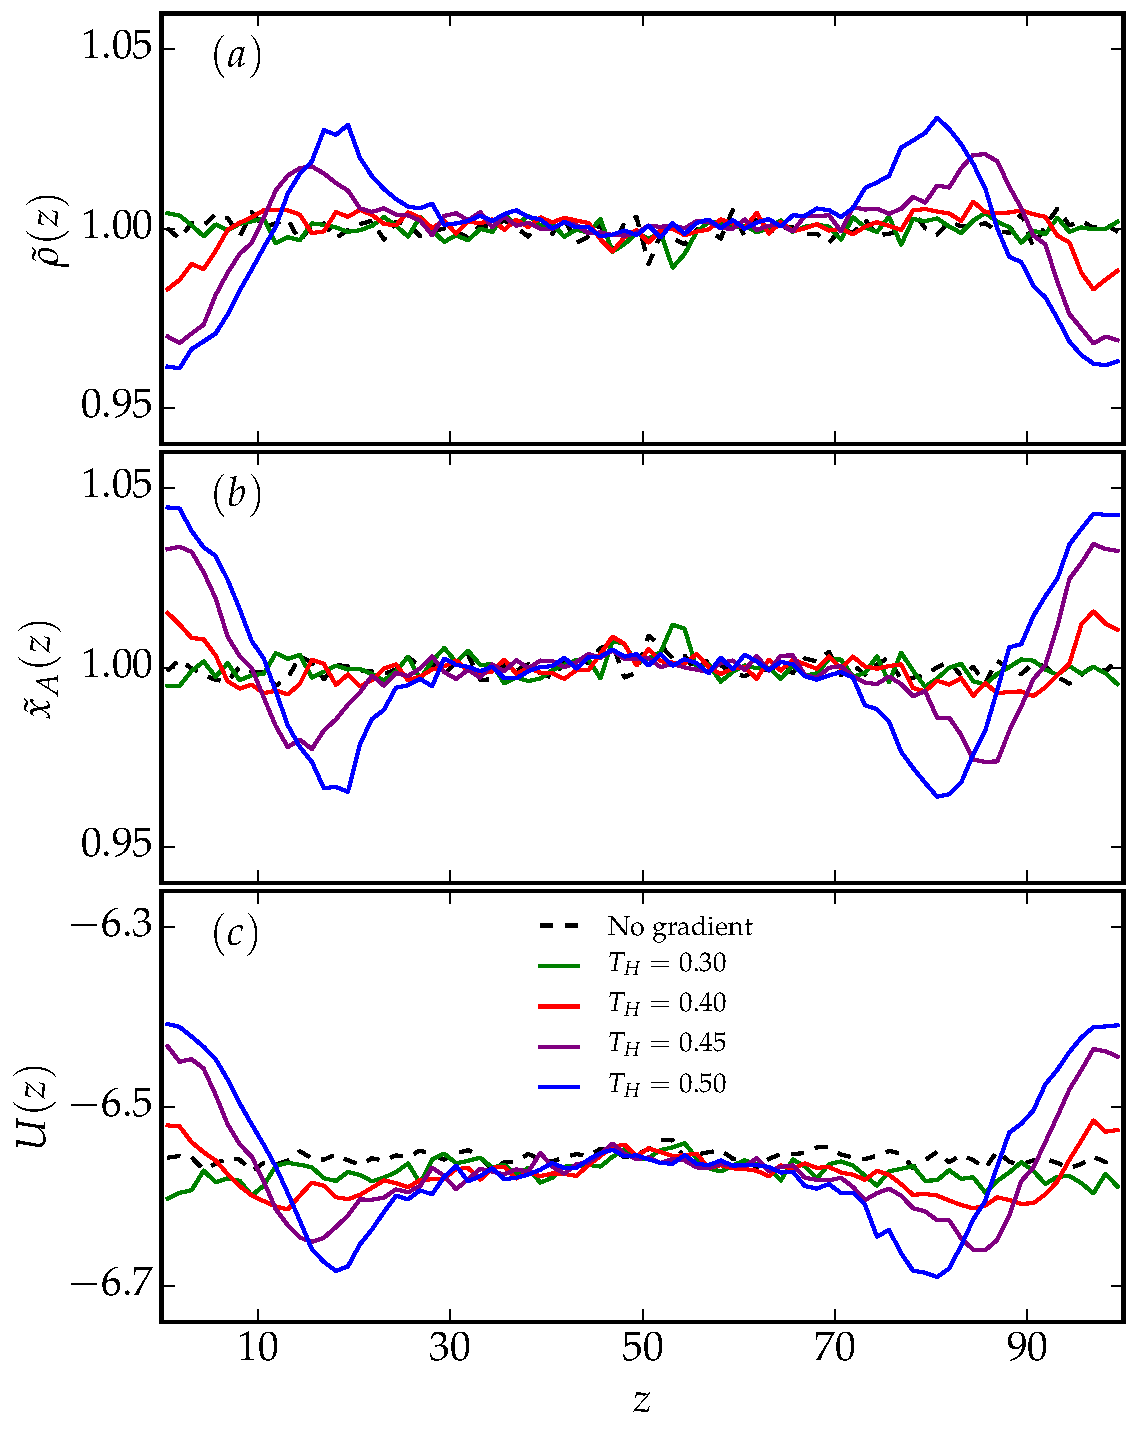
\includegraphics[width=7cm]{./figs/thermalResponse.pdf}
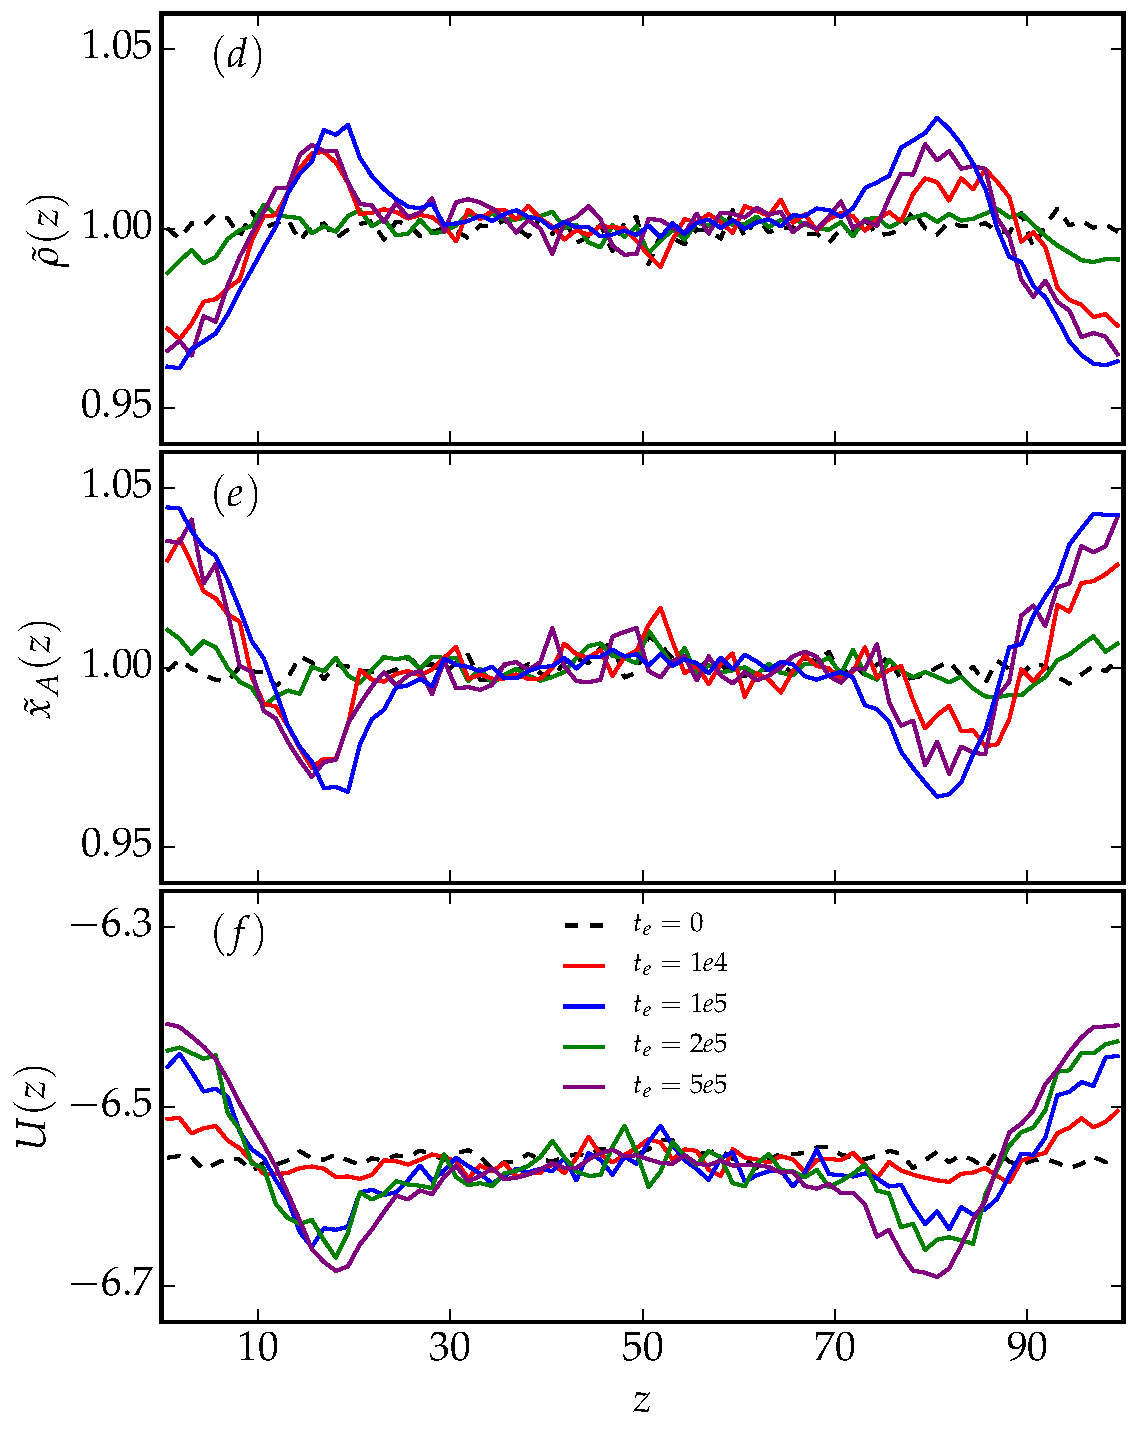
\includegraphics[width=7cm]{./figs/thermalResponse_exp.pdf}
\caption[{\em Thermal processing: applying thermal gradient to prepare inhomogeneous glassy samples}]{{\em Response to thermal gradient pulse.} Measurement of spatial profiles of normalized density $\tilde{\rho}_A(z)$,  normalized concentration of larger species $\tilde{x}_A(z)$ and potential energy $U(z)$ in the $z$-direction are shown after switching off the gradient after a period of $t_{\rm exp} = 5\times10^5$. Subsequently, these profiles are sampled over a period of $5\times10^4$. (a-c) Spatial profiles are shown for different temperature gradients: $T_C = 0.20$ and $T_H = 0.30, 0.40, 0.45, 0.50$, including the case which has been exposed to the temperature gradient. (d-f) Spatial profiles are shown for a fixed temperature gradient $T_C = 0.20$ and $T_H = 0.50$ but exposure time of $t_{\rm exp} = 10^4, 10^5, 2\times10^5, 5\times10^5$.}
\label{thermal}
\end{figure*}
%%%%%%%

As outlined above, the inhomogeneous glassy samples are prepared via the protocol mentioned in the methods section of this chapter (very similar to the discussion on the response to a thermal gradient pulse, discussed in previous chapter). The samples are exposed to a thermal gradient pulse such that the temperature of cold zone is maintained at $T_C = 0.2$ and the temperature of hot zone is maintained at $T_H = 0.3,0.4, 0.45, 0.5$, for a period of $t_{\rm exp}$. After this period, the gradient is switched off by having both the zones at the same temperature $T_H = T_C = 0.2$, for a period of $5 \times 10^4$. Below, we discuss the changes in the spatial properties of the glassy samples before the gradient exposure and after the gradient exposure. 
 
 For convenience, as in the previous chapter, we define normalized local density and concentration as $\tilde{\rho}(z)\equiv\rho(z)/\bar{\rho}$ and $\tilde{x}_A(z)\equiv x_A(z)/\bar{x}_A$, where $\rho(z)$ is the local number density, $x_A$ is the local concentration of A-species and the global parameters $\bar{\rho}$ and $\bar{x}_A$ are the average number density and average concentration of A-species with values $1.2$ and $0.8$ respectively. 
 
 The aged glassy sample, in the absence of the thermal protocol discussed above, is expected to have no spatial variation of $\tilde{\rho}(z)$, $\tilde{x}_A(z)$ and local potential energy $U(z)$, as shown with the dotted black line in Fig.~\ref{thermal}. But when the gradient is on, the region where the local temperature is high will start relaxing (and even melting for $T > T_{MCT}$) with relatively higher mobility, leading to local structural changes. These changes will keep evolving until the gradient is on. But as soon as gradient is switched off and the sample is back to a glassy environment, the evolving structural changes almost freeze \cite{vaibhav2020response} to provide an inhomogeneous glassy sample with spatial variation of $\tilde{\rho}(z)$, $\tilde{x}_A(z)$ and $U(z)$. These spatial measurements done over a period of $5 \times 10^4$, after switching off the gradient, are shown in Fig.~\ref{thermal}. Moreover, we have checked the aging process of these profiles, and this is found to be extremely slow. This is expected because after the thermal gradient is switched off, the whole sample instantaneously returns back to a glassy environment at temperature $T_C = 0.2$, causing extreme difficulty for any structural rearrangements.  
 
 In the left panel of Fig.~\ref{thermal}(a-c), measurements are shown after applying the different thermal gradients ($T_C = 0.2$ and $T_H = 0.3,0.4,0.45,0.5$) for a period of $t_{\rm exp} = 5\times 10^5$. The spatial variation in the profiles becomes more prominent if the gradient is bigger. If we look at the normalized density (Fig.~\ref{thermal}a), we find that the local relaxation or melting near the hotter ends causes local expansion of the material leading to local decrease in density. This leads to the regions close to hotter regions being pushed due to expansion, leading to increase in density. On the other hand, since the middle of the material is always at $T_C = 0.2$, so the density is roughly not affected, for the used timeline of thermal protocol. Next, we analyse the concentration variation happening in the sample, as shown in Fig.~\ref{thermal}b. The temperature gradient affects the bigger and smaller particles differently which causes concentration imbalance. As we see here, bigger particles have high concentration near the hotter ends which shows the tendency of these particles to move in the direction of thermal gradient, unlike the smaller particles which prefer to move opposite to the thermal gradient applied. This local melting causes local structural changes in the material which can be seen in the local measurements of potential energy (Fig.~\ref{thermal}c). Locally high temperature near the hotter region has relatively higher potential energy, meaning these regions tries to achieve the corresponding high temperature state of higher potential energy. The immediate neighbouring region has relatively lower potential energy because of the compression, as discussed above.
 
 In the right panel of Fig.~\ref{thermal}, we show the spatial variation of the quantities measured after applying the thermal gradient by having $T_C = 0.2$ and $T_H = 0.5$ for a period of $ t_{\rm exp} = 10^4, 10^5, 2\times10^5, 5\times10^5$. Again, these spatial measurements are done over a period of  $5 \times 10^4$ after switching off the gradient. It is very clear that the heterogeneity in terms of local density, local concentration and local potential energy, increases with the increase in the exposure time of the gradient. Longer exposure keep the melting process near the hotter end on, resulting in to the increase of the heterogeneity. Such development of heterogeneity is happens rapidly when the gradient is switched on but the process becomes very slow after some time.
 
 So, we have been able to prepare inhomogeneous glassy samples which we call {\em thermally processed samples} or {\em thermally treated samples}, by exposing the freshly prepared glassy states to thermal gradient pulse. The degree of heterogeneity in these samples can be controlled by varying the thermal gradient applied and also by tuning the exposure time for which the thermal gradient is active. 
 

\subsection{Shear response of thermally processed samples}

 %%%%%%%%%
\begin{figure*}[hbt!]
\centering
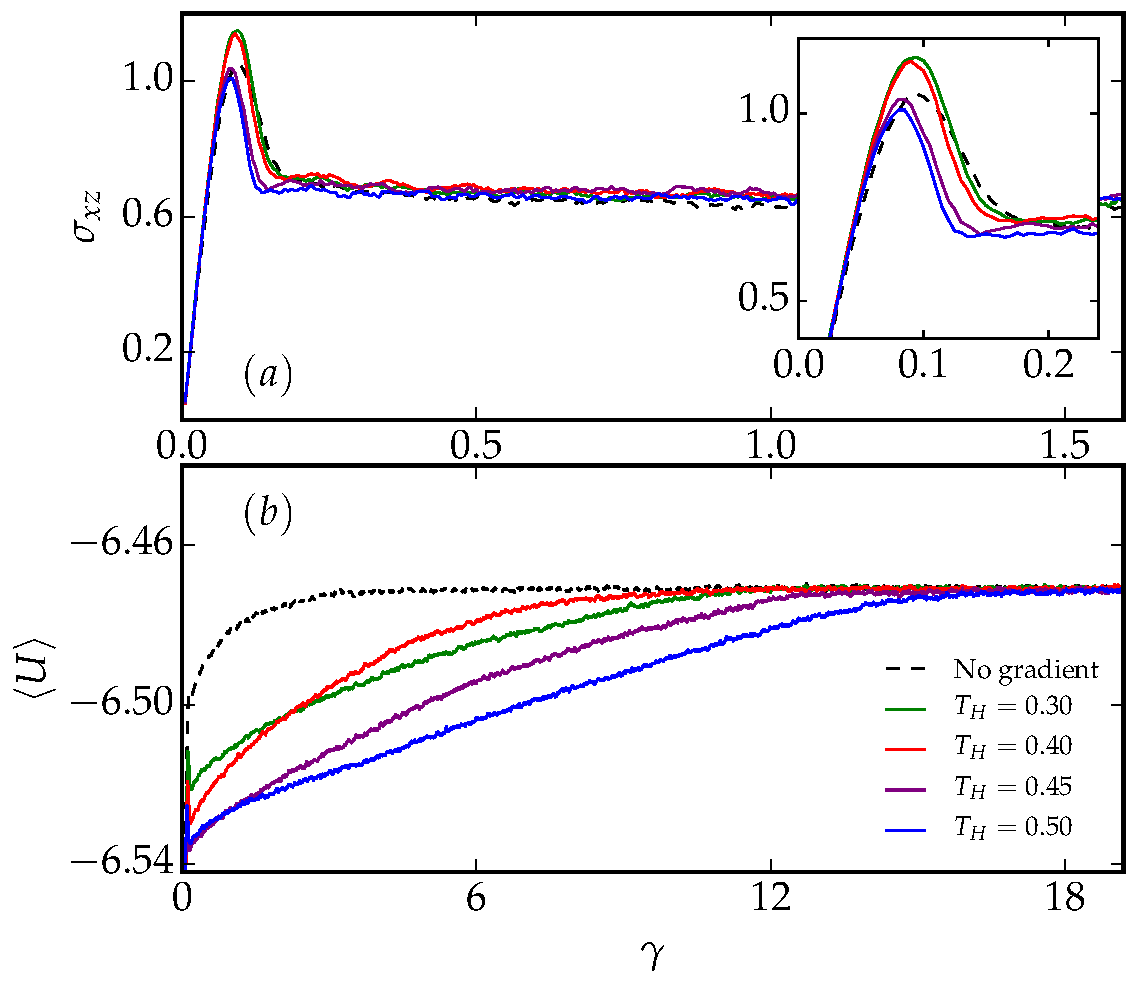
\includegraphics[width=10.2cm]{./figs/shearResponse.pdf}
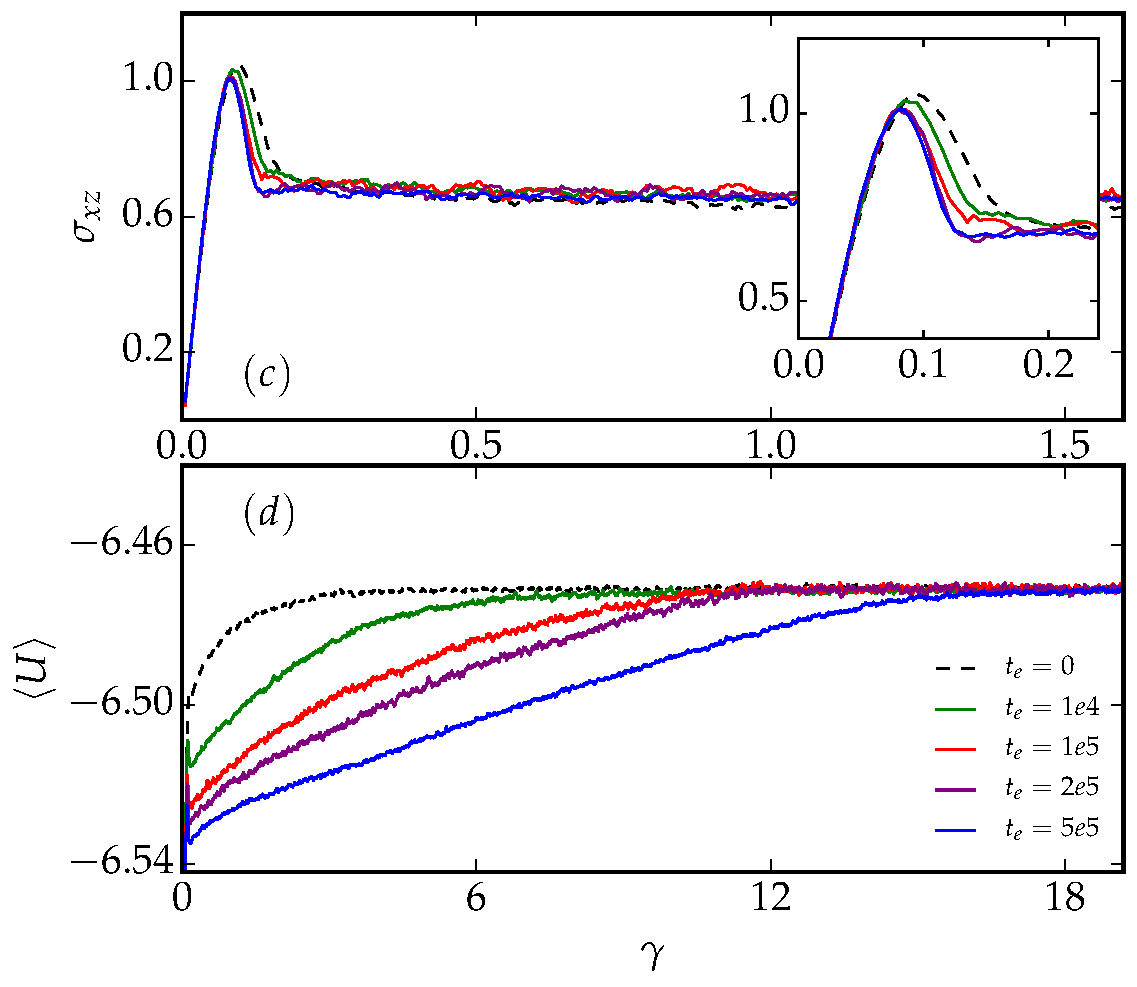
\includegraphics[width=10.2cm]{./figs/shearResponse_exp.pdf}
\caption[{\em Shear response of thermally processed inhomogeneous glassy states.}]{{\em Shear response of thermally processed inhomogeneous glassy states.} Shear stress $\sigma_{xz}$ and potential energy $\langle U \rangle$ are shown when system is sheared with shear-rate $\dot{\gamma} = 10^{-3}$. (a-b) Measurements are shown for samples processed through different temperature gradients: $T_C = 0.20$ and $T_H = 0.30, 0.40, 0.45, 0.50$, including the case which has been exposed to the temperature gradient. (c-d) Measurements are shown for samples processed through a fixed temperature gradient $T_C = 0.20$ and $T_H = 0.50$ but exposure time (time for which gradient was on) of $t_{\rm exp} = 0, 10^4, 10^5, 2\times10^5, 5\times10^5$.}
\label{shear}
\end{figure*}
%%%%%%%

As described above, we obtain thermally processed glassy samples with spatial inhomogeneity in $z$-direction, the direction in which thermal gradient is applied. These samples are sheared in the $x$-direction by deforming the $xz$-plane with fixed shear rate $\dot{\gamma}$ so that the density heterogeneity in the $z$-direction is part of flow gradient direction. Our goal is to compare the shear response of the inhomogeneous glassy samples with that of the sample which has not been exposed to the thermal gradient. We measure the stress-strain behaviour and the evolution of average potential energy  $\langle U \rangle$ of the system with strain (see Fig.~\ref{shear}) for thermally processed (shown with solid lines in Fig.~\ref{shear}) and unprocessed samples (shown with dotted black line in Fig.~\ref{shear}). The shear stress $\sigma_{xz}$ is calculated using the following Irving-Kirkwood expression: 
    \begin{equation}
        \sigma_{xz} = \langle \frac{1}{V} \sum_{\alpha\beta} f^{x}_{\alpha\beta} r^{z} \rangle,
    \end{equation}
where $f^{x}_{\alpha\beta}$ is the $x$-component of the force with respect to a pair of particles and $r^z$ is the $z$-component of the distance vector between two particles labelled $\alpha$ and $\beta$ which could belong to either of the species A and B. $V$ is the total volume of the simulated system. $\langle\cdot\rangle$ corresponds to averaging over independent samples.
    
A typical glassy system under shear responds elastically with the linear increase in stress for small deformation followed by a stress overshoot and then homogeneous flow in long time when steady state is achieved. Similarly, the average potential energy increases initially and goes to a steady value in long time. In Fig.~\ref{shear}, results have been shown for sheared system with shear rate $10^{-3}$ in Fig.~\ref{shear}(a-b) with varying thermal gradient and in Fig.~\ref{shear}(c-d) for a given gradient but varying the exposure time of the gradient.

If we look at the stress vs strain ($\sigma_{xz}$ vs $\gamma$) plots in Fig.~\ref{shear}a, initial increase of stress is almost similar for both processed and unprocessed samples, meaning the modulus of the material is not much affected. But with the increase in strain, the behaviour of processed samples, which had $T_H > T_{MCT}$, start to be different from the unprocessed samples. The height in the stress overshoot of these samples, as seen in the inset, decrease with the increase in inhomogeneity, i.e. they have a softer response. But for smaller gradients, where $T_H = 0.3, 0.4$,  stress overshoot has values even higher than the unprocessed samples (see inset of Fig.~\ref{shear}a), implying that their response is more rigid. After yielding, the stress drops over a window of strain which decreases with the increase in inhomogeneity. This indicates the failure process in such materials becomes sharper.% if the inhomogeneity is increased \cite{ozawa2018random}. 
This will become more evident when we probe the failure mechanism in such materials at microscopic level. Similarly, if the exposure time is varied keeping the thermal gradient fixed, with the increase in exposure time, the stress drops after the overshoot over a shorted strain window (see Fig.~\ref{shear}c and the corresponding inset). Hence, with the increase in heterogeneity, either due to increase in the thermal gradient or due to increase in the exposure time, the stress drop becomes sharper. %, meaning the failure becoming localized.

Next we study the evolution of $\langle U \rangle$ with strain, shown in Fig.~\ref{shear}b and Fig.~\ref{shear}d. We observe that the steady state for thermally processed samples is achieved at relatively large values of strain i.e., $10$ to $15$ times the value of the strain at which the steady state is achieved for unprocessed samples. Also, as the thermal gradient is increased or exposure time is increased, the time scale to reach steady state also increases.  This means that the time scale of obtaining the steady state has one to one correspondence with the level of heterogeneity. % because we have already seen in Fig.~\ref{thermal}, the heterogeneity of the sample increases with the increase in thermal gradient and also with the increase in the exposure time of the thermal gradient. 
This increase in timescale to attain steady state with the increase in inhomogeneity is expected.% because steady state means the homogeneous flow of the material, which will happen in thermally processed inhomogeneous materials at later times. 
Shear will try to homogenize the material once steady state has been reached. However, this happens relatively quickly in unprocessed samples. On the other hand, the homogenization process slows down with the increase in spatial inhomogeneity in the initial glassy state.

\subsection{Nucleation and evolution of shear bands}

%%%%%%%%%
\begin{figure}[hbt!]
\centering
\includegraphics[width=13cm]{./figs/mobMap_tempGrad.pdf}
\caption[{\em Mobility maps of sheared thermally processed samples: impact of gradient}]{{\em Mobility maps of sheared thermally processed samples: impact of gradient.} Different temperature gradient pulses with $T_C = 0.20$ and $T_H = 0.30, 0.40, 0.50$ (also marked), are applied for $t_{\rm exp} = 2\times10^5$ to generate inhomogeneous glassy samples and then these samples are sheared with shear rate $\dot{\gamma} = 10^{-4}$. These maps are constructed using non-averaged single particle squared displacement in $z$-direction, assuming time at the start of the shear as origin. Upper panel (a) maps are shown for the case of unprocessed samples. Maps on the left side of the vertical line show the evolution of shear bands with strain $\gamma = 0.1, 0.5, 1.0, 2.0, 5.0$ (also marked), while maps on right side are shown at the fixed value of strain $\gamma = 4.0$ and starting with the same thermally processed sample but different random seed for DPD thermostat.}
\label{mapVaryGrad}
\end{figure}
%%%%%%%


In the previous section, we have analysed the macroscopic rheological response of inhomogeneous glassy samples. Now, we examine the inhomogeneous flow patterns at microscopic level of these samples, during the response to the applied shear. For this purpose, for a chosen initial state, we compute the mobility  maps using  single particle squared displacement $\delta r^2_z(t)$, measured with respect to the state at $t=0$, i.e. at the start of shear. These maps have been calculated at different strain values, using an imposed shear rate of $10^{-4}$; see Fig.~\ref{mapVaryGrad} and \ref{mapVaryExp}. The flow behaviour in terms of such mobility maps has been used in earlier studies \cite{golkia2020} to probe the emergence and evolution of the flow heterogeneities in the form of shear-bands. Here, we compare the flow patterns via the mobility maps, for both thermally processed and unprocessed samples.

In Fig.~\ref{mapVaryGrad}, we present the shear bands at the different strain values, for the untreated glassy samples (Fig.~\ref{mapVaryGrad}a) and  glassy samples treated via different temperature gradients ($T_C = 0.20 $ and $T_H = 0.30, 0.40, 0.50$) (Fig.~\ref{mapVaryGrad}(b-d)), as discussed above. On the left side of the vertical line in Fig.~\ref{mapVaryGrad}, shear bands have been shown at strain values $0.1, 0.5, 1.0, 2.0, 5.0$. In the unprocessed sample, at small strains, very weak shear band is formed from hot spots at random locations, and these gets spatially homogenized at a strain value of $4.0$. But inhomogeneous samples show very sharp localized band patterns, at early strain. The expansion of these shear bands become slower or the lifetime of shear bands become longer for bigger gradients, this can be observed visually by comparing the bands at a particular strain value for different thermal gradients. This observation is consistent with the macroscopic observations made above, viz. with the increase in spatial inhomogeneity in the gradient direction, the sample takes longer time for reach a spatially homogeneous steady state. We also note that for $T_H = 0.3, 0.4$, the band (faster region) nucleates in the middle of the sample, near the colder end, and it expands towards the hotter region, while for $T_H = 0.5$ the band nucleation happens near the hotter region and it expands towards the colder region. The difference in the location of the shearband formation could be due to relative local stability due to the spatial heterogeneity in the initial state.

Similarly, in Fig.~\ref{mapVaryExp}(a-d), we present the shear bands at the different strain values for the glassy samples treated using a fixed thermal gradient ($T_C = 0.2 $ and $T_H = 0.50$) but different exposure time $t_{\rm exp} = 0, 10^3, 10^4, 10^5$. In this case, the main observation is the lifetime of the band increases with the increase in the time window over which the initial states were exposed to the thermal gradient. This observation is consistent with the macroscopic measurements in Fig.~\ref{shear}d, where we observed that the timescale of reaching steady state increases with the increase in exposure time . The location of shear band is roughly the same in all cases of finite exposure time in Fig.~\ref{mapVaryExp}(b-d), similar to the case of Fig.~\ref{mapVaryGrad}d where the same gradient is applied for $t_{\rm exp} = 2\times10^5$ i.e., shear band always nucleates near the extreme ends close to hotter region.

%%%%%%%%%
\begin{figure}[hbt!]
\centering
\includegraphics[width=13cm]{./figs/mobMap_tExp.pdf}
\caption[{\em Mobility maps of sheared thermally processed samples: impact of exposure time}]{{\em Mobility maps of sheared thermally processed samples: impact of exposure time.} A fixed temperature gradient pulse with $T_C = 0.20$ and $T_H = 0.50$ is applied for different duration $t_{\rm exp} = 0, 10^3, 10^4, 10^5$ (also marked) to generate inhomogeneous glassy samples and then these samples are sheared with shear rate $\dot{\gamma} = 10^{-4}$. These maps are constructed using using non-averaged single particle squared displacement in $z$-direction, assuming time at the start of the shear as origin. Upper panel (a) maps are shown for the case of unprocessed samples. Maps on the left side of the vertical line shows the evolution of shear bands with strain $\gamma = 0.1, 0.5, 1.0, 2.0, 5.0$ (also marked), while maps on right side are shown at the fixed value of strain $\gamma = 4.0$ and starting with the same thermally processed sample but different random seed for DPD thermostat.}
\label{mapVaryExp}
\end{figure}
%%%%%%%


%{\em Inhomogeneity decides the nucleation and growth of shear bands.} 
Finally, we demonstrate that the location of the density inhomogeneities in the initial sample, prior to shear, determines the location of the flow bands observed during the shear.
%Up to now we have seen the macroscopic and microscopic mechanism of failure is different in thermally processed inhomogeneous samples, compared with the glassy samples which are not exposed to any thermal gradient. In particular, we observed very special flow patterns in the shear response of these samples i.e., depending on the gradient used to treat the sample the shear band nucleation can be near the hotter region or colder region. Now, we want to understand the role of inhomogeneity in the determination of location of nucleation of shear band and its growth. 
For this purpose, we start with an inhomogeneous glassy sample obtained after switching off the gradient and perform at least $10$ different shear deformation simulations with $\dot{\gamma} = 10^{-4}$, using different random seed for the DPD thermostat which maintains the temperature at $0.2$. Hence, in each simulation, the spatial heterogeneity of the sample is same but the random kicks faced by particles during deformation are different. 
%Such analysis will help us in understanding the role of inhomogeneity in the determination of mode of failure. 
Next, we show on the right side of vertical line in Fig.~\ref{mapVaryGrad}, the mobility map at the strain value of $\gamma = 4.0$ for $10$ different simulations with same initial inhomogeneity at the start of deformation . In all samples, except for the case of a few samples at $T_H = 0.4$, mobility maps show similar  pattern, i.e., for $T_H = 0.3, 0.4$ shear band nucleates close to the colder region and expands towards the hotter region and for $T_H = 0.5$ shear band always nucleates near the hotter region at extreme ends and then expands towards the colder region. This is in contrast to the unprocessed sample where the slower regions are located at different levels along $z$, which is consistent with previous observations \cite{golkia2020}. Therefore, for the processed samples, we can conclude that there is no run-to-run variation, i.e. there is no stochastic effect is the selection of the location unlike the case of the unprocessed states \cite{golkia2020}. Hence, this selection of the location of shearband formation must be related to features in the initial structure. A similar exercise is also done for the case of samples having different exposure time; see right column of Fig.\ref{mapVaryExp}. There too we observe no run to run variation, specially for samples which have been exposed to the thermal gradient for long times. 

\section{Conclusions}

We have studied the shear response of inhomogeneous glassy samples prepared by exposing homogeneous glassy states to a thermal gradient pulse. Our aim is to understand whether the mechanical behaviour, specially the spatial response, is influenced by the initial structural heterogeneities. 


First, we have characterised the spatial inhomogeneity, generated via the thermal protocol discussed above, in terms of spatial profiles of density, concentration and local potential energy. We observe that the degree of heterogeneity is controlled by the applied thermal gradient and its exposure time. 

%We have investigated the failure mechanism in heterogeneous samples obtained by changing the thermal gradient for fixed exposure time and by changing the exposure time for a fixed gradient.

Next, the mechanical response was studied by driving these samples by a fixed shear-rate. We observe that the timescale at which the sheared inhomogeneous states achieve steady state is delayed, in comparison with the initial homogeneous glassy states, which is related to the slow flow homogenization within the samples. The microscopic insights of this failure mechanism in deformed inhomogeneous glassy samples is thereafter obtained via mobility maps. This analysis suggests that it is possible to have a control over the location of the failure via the initial spatial heterogeneity in the glassy state. In particular, location of shear band initiation has one-to-one correspondence with the heterogeneity in the sample, which is confirmed by a thought experiment involving the stochasticity of the thermostat vis-a-vis a single heterogeneous sample and showing that stochasticity has no role to play in the location of the shearband. 

The extension of this project should be to perform simulation studies at very low temperatures, where some interesting features are expected. Also, a computer experiment can be performed where different kinds of thermal pulses can be utilised to generate more variations in spatial heterogeneity aimed at targeted design. Further, other shear directions can be explored to understand the failure mechanism and its coupling to these heterogeneities.